\documentclass[aps, pre, onecolumn, nofootinbib, notitlepage, groupedaddress, amsfonts, amssymb, amsmath]{revtex4-1}
%%%%%%begin preamble
\usepackage[hmargin=1in, vmargin=1in]{geometry} % Margins
\usepackage{hyperref}
\usepackage{url}
\usepackage{natbib}
\setlength{\bibsep}{0pt plus 0.3ex}
\usepackage{graphicx}
%\usepackage{pdfpages} % breaks with aastex6
\usepackage{import}
\usepackage{wrapfig}

\usepackage{xcolor}
\hypersetup{
  colorlinks   = true,
  %citecolor    = blue
  citecolor    = gray
  % gray is not being found!?!
  % gray is found if pdfpages is used... crap.
  %citecolor    = grey
  %citecolor    = Gray
}

%Copy+pasted from aastex.
\newcommand\aj{\ref@jnl{AJ}}%        % Astronomical Journal 
\newcommand\araa{\ref@jnl{ARA\&A}}%  % Annual Review of Astron and Astrophys 
\renewcommand\apj{\ref@jnl{ApJ}}%    % Astrophysical Journal ++
\newcommand\apjl{\ref@jnl{ApJL}}     % Astrophysical Journal, Letters 
\newcommand\apjs{\ref@jnl{ApJS}}%    % Astrophysical Journal, Supplement 
\renewcommand\ao{\ref@jnl{ApOpt}}%   % Applied Optics ++
\newcommand\apss{\ref@jnl{Ap\&SS}}%  % Astrophysics and Space Science 
\newcommand\aap{\ref@jnl{A\&A}}%     % Astronomy and Astrophysics 
\newcommand\aapr{\ref@jnl{A\&A~Rv}}%  % Astronomy and Astrophysics Reviews 
\newcommand\aaps{\ref@jnl{A\&AS}}%    % Astronomy and Astrophysics, Supplement 
\newcommand\azh{\ref@jnl{AZh}}%       % Astronomicheskii Zhurnal 
\newcommand\baas{\ref@jnl{BAAS}}%     % Bulletin of the AAS 
\newcommand\icarus{\ref@jnl{Icarus}}% % Icarus
\newcommand\jrasc{\ref@jnl{JRASC}}%   % Journal of the RAS of Canada 
\newcommand\memras{\ref@jnl{MmRAS}}%  % Memoirs of the RAS 
\newcommand\mnras{\ref@jnl{MNRAS}}%   % Monthly Notices of the RAS 
\renewcommand\pra{\ref@jnl{PhRvA}}% % Physical Review A: General Physics ++
\renewcommand\prb{\ref@jnl{PhRvB}}% % Physical Review B: Solid State ++
\renewcommand\prc{\ref@jnl{PhRvC}}% % Physical Review C ++
\renewcommand\prd{\ref@jnl{PhRvD}}% % Physical Review D ++
\renewcommand\pre{\ref@jnl{PhRvE}}% % Physical Review E ++
\renewcommand\prl{\ref@jnl{PhRvL}}% % Physical Review Letters 
\newcommand\pasp{\ref@jnl{PASP}}%     % Publications of the ASP 
\newcommand\pasj{\ref@jnl{PASJ}}%     % Publications of the ASJ 
\newcommand\qjras{\ref@jnl{QJRAS}}%   % Quarterly Journal of the RAS 
\newcommand\skytel{\ref@jnl{S\&T}}%   % Sky and Telescope 
\newcommand\solphys{\ref@jnl{SoPh}}% % Solar Physics 
\newcommand\sovast{\ref@jnl{Soviet~Ast.}}% % Soviet Astronomy 
\newcommand\ssr{\ref@jnl{SSRv}}% % Space Science Reviews 
\newcommand\zap{\ref@jnl{ZA}}%       % Zeitschrift fuer Astrophysik 
\renewcommand\nat{\ref@jnl{Nature}}%  % Nature 
\newcommand\iaucirc{\ref@jnl{IAUC}}% % IAU Cirulars 
\newcommand\aplett{\ref@jnl{Astrophys.~Lett.}}%  % Astrophysics Letters 
\newcommand\apspr{\ref@jnl{Astrophys.~Space~Phys.~Res.}}% % Astrophysics Space Physics Research 
\newcommand\bain{\ref@jnl{BAN}}% % Bulletin Astronomical Institute of the Netherlands 
\newcommand\fcp{\ref@jnl{FCPh}}%   % Fundamental Cosmic Physics 
\newcommand\gca{\ref@jnl{GeoCoA}}% % Geochimica Cosmochimica Acta 
\newcommand\grl{\ref@jnl{Geophys.~Res.~Lett.}}%  % Geophysics Research Letters 
\renewcommand\jcp{\ref@jnl{JChPh}}%     % Journal of Chemical Physics 
\newcommand\jgr{\ref@jnl{J.~Geophys.~Res.}}%     % Journal of Geophysics Research 
\newcommand\jqsrt{\ref@jnl{JQSRT}}%   % Journal of Quantitiative Spectroscopy and Radiative Trasfer 
\newcommand\memsai{\ref@jnl{MmSAI}}% % Mem. Societa Astronomica Italiana 
\newcommand\nphysa{\ref@jnl{NuPhA}}%     % Nuclear Physics A 
\newcommand\physrep{\ref@jnl{PhR}}%       % Physics Reports 
\newcommand\physscr{\ref@jnl{PhyS}}%        % Physica Scripta 
\newcommand\planss{\ref@jnl{Planet.~Space~Sci.}}%  % Planetary Space Science 
\newcommand\procspie{\ref@jnl{Proc.~SPIE}}%      % Proceedings of the SPIE 

\newcommand\actaa{\ref@jnl{AcA}}%  % Acta Astronomica
\newcommand\caa{\ref@jnl{ChA\&A}}%  % Chinese Astronomy and Astrophysics

\setcounter{tocdepth}{2}
%% headers
\usepackage{fancyhdr}
\pagestyle{fancy}
\fancyhf{} % sets both header and footer to nothing
\lhead{Evan Anders---Research Statement}
\rhead{Stanford University, Stanford Science Fellows}
\cfoot{\footnotesize{\thepage}}
%\pagestyle{empty}
%\pagenumbering{gobble}
%\renewcommand*{\thefootnote}{\fnsymbol{footnote}}

\renewcommand{\vec}{\ensuremath{\boldsymbol}}
\newcommand{\dedalus}{\href{http://dedalus-project.org}{Dedalus}}
\newcommand{\del}{\ensuremath{\vec{\nabla}}}
\newcommand{\scrS}{\ensuremath{\mathcal{S}}}

\newcommand{\nosection}[1]{%
  \refstepcounter{section}%
  \addcontentsline{toc}{section}{\protect\numberline{\thesection}#1}%
  \markright{#1}}
\newcommand{\nosubsection}[1]{%
  \refstepcounter{subsection}%
  \addcontentsline{toc}{subsection}{\protect\numberline{\thesubsection}#1}%
  \markright{#1}}

%\usepackage{atbegshi}
%%%%%%end preamble


\begin{document}
\section*{Motivation and Research Problem}
\vspace{-11pt}
Stars are the cornerstone of studies in astrophysics.
Starlight is used to detect exoplanets and sample the composition of interstellar space, and stars are the progenitors of exotic objects like black holes.
Despite being intricately linked to studies across astrophysics, stars are fascinating experiments in magnetism and fluid dynamics in and of themselves.
My research interests focus on stars like the Sun, which rely on vigorous near-surface convective regions to transport the heat generated in their cores.
This convection generates sound waves which refract due to density stratification as they propagate into the stellar interior.
The relatively new field of asteroseismology measures the wave patterns at the stellar surface to learn about the interior structure of stars.
These measurements enable the precise determination of age, mass, and radius of many stars; furthermore, high resolution ``helioseismic'' observations of the Sun have revealed the interior structure and flows of our nearest star.
It is theorized that large-scale convective flows called ``giant cells'' should be present in stars like the Sun, but helioseismic observations and direct measurements have been unable to detect them.
The absence of these flows has called into question our most fundamental understanding of the nature of convection in stars, a problem widely referred to as the ``Solar Convective Conundrum.''

The Convective Conundrum is troubling not only for modelers of stellar convection, but also for anyone who studies asteroseismology or relies on asteroseismic results.
Models of stellar interiors are essential for the interpretation of asteroseismic and helioseismic data, but state-of-the-art codes which generate these structure models rely on one-dimensional (1D) parameterizations of convection.
The 1D parameterizations that inform these codes assume giant cells exist in the Sun, and this assumption conflicts with modern observations.

My research aims to  help solve this Convective Conundrum by gaining a better understanding of convection in the highly stratified, rotating, magnetized context of stellar convection.
During my time at Stanford, I will conduct a series of studies which will span from the smallest to the largest scales present in stellar convection.
I will use the understanding gained in detailed, small-scale studies to inform the interpretation of large-scale global studies.
While I draw my inspiration from problems facing the solar and stellar community, similar flow processes may be important in the atmospheres and cores of planets like Jupiter and the Earth. 


\vspace{-10pt}
\section*{Research Plan}
\vspace{-11pt}
\paragraph*{The smallest convective scales: individual downflows}
\begin{wrapfigure}{r}{0.22\textwidth}
	\begin{center}
	\vspace{-25pt}
    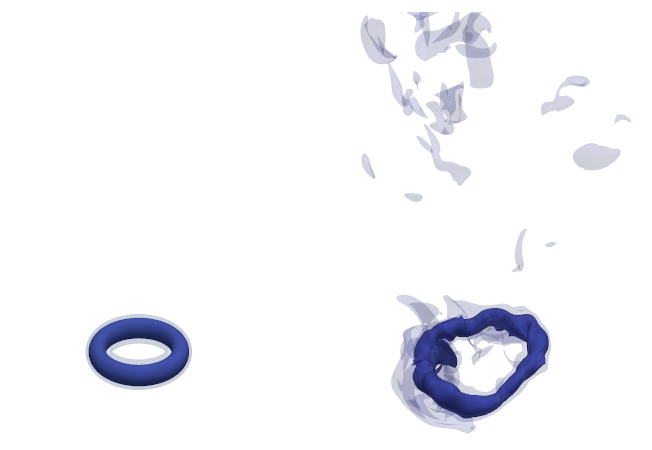
\includegraphics[width=0.21\textwidth]{./figs/thermals_comparison.png}
	\vspace{-20pt}
	\end{center}
    \caption{
	3D visualizations of entropy perturbations in the downward-propagating reference frame of evolved laminar (left) and turbulent (right) thermals.
	\label{fig:thermals_comparison} }
	\vspace{-11pt}
\end{wrapfigure}
The density stratification present in stars makes stellar convection exhibit upwellings that are slow, weak, and wide in balance with downflows which are intense, fast, and narrow.
It has been hypothesized that downflows may be so powerful in the context of solar-like convection that they alone transport the Sun's luminosity.
These downflows would exist alongside mass-conserving upflows which exhibit negligible energy transport.
This ``entropy rain'' hypothesis, first suggested by \citet{spruit1997}, is gaining traction in recent simulations \cite{kapyla&all2017} and theoretical work \citep{brandenburg2016}, and could explain the absence of giant cells in observations \citep{hanasoge&all2015}.
It is possible these downflows turbulently break up into distinct pieces as they fall and these individual downflow pieces can be well modeled as ``thermals.''
Thermals are regions of cold fluid which accelerate due to buoyancy forces and shape themselves into vortex rings; evolved thermals are visualized in Fig. \ref{fig:thermals_comparison}.
Thermals are also observed and studied in the Earth's atmosphere \citep{lecoanet&jeevanjee2019}.

As a Stanford fellow, I will build upon my previous study of thermals \citep{andersLB2019} to understand if entropy rain is feasible.
The interactions of rotation, magnetism, and turbulence could filter downflows and prevent their successful transit of the solar convection zone in certain regimes, but the importance of these effects on thermals has not yet been studied.
I will determine whether strong magnetic fields and global rotation can ``evaporate'' entropy rain.

\paragraph*{Intermediate-scale convection: interactions at the radiative-convective boundary}
In Sun-like stars, the turbulent convection zone lies above a stably stratified ``radiative zone'' where radiation effectively carries the stellar luminosity.
In the Sun, the radiative-convective boundary (RCB) is characterized by a transition from moderate instability to strong stability.
The solar RCB furthermore coincides with a region of intense shear in the Sun's radial velocity profile called the tachocline, and it is thought that these shear interactions are a crucial driver of the Sun's magnetic dynamo.
Understanding how downflows pump angular momentum and magnetism into the RCB is crucial to figuring out how the solar dynamo is driven, and how the tachocline was established.
Measurements suggest that the RCB is thin \citep{basu1997}, but many modern simulations produce RCBs which are up to an order of magnitude thicker than the solar one \citep{hotta2017}.
This suggests that many simulations are studying angular momentum and magnetic field pumping mechanisms in the wrong regime of ``stiffness'' of the RCB \citep{couston&all2017}.

During my time at Stanford, I will study how an ensemble of downflows interacts with a solar-like RCB in the presence of solar-like rotation and magnetism.
I will study simulations of localized, solar-like, rotating magnetoconvection and determine if downflows can effectively pump magnetic fields and angular velocity into a thin, solar-like RCB.

\paragraph*{Global scale convection: dynamics in relaxed atmospheres}
Modern 1D stellar models often employ the decades-old convective parameterization of mixing length theory \citep{bohm-vitense1958}, which has many deficiencies.
These deficiencies have led some researchers to seek out ways to couple 1D models with fully convective, three-dimensional (3D) global simulations.
Such a coupling has recently been performed with some success \citep{jorgensen&weiss2019}, but the 3D simulations utilized were localized in a very thin layer near the stellar surface.
Furthermore, \citet{jorgensen&weiss2019} coupled previously computed 3D simulations with 1D models, rather than coupling the two at runtime, largely because 3D simulations are costly.
Some of these costs are unavoidable: highly resolved, turbulent simulations necessarily take small timesteps, and therefore simulation times are very long.
Thin, near-surface simulations such as those used by \citet{jorgensen&weiss2019} examine a regime where the convective overturn timescale is very similar to the local Kelvin-Helmoltz (KH) timescale of atmospheric equilibration.
In studies of deep convection these timescales become disparate, and many overturn timescales pass during one KH timescale.
Thus, much of the expense of simulations which include deep convection is often time ``wasted'' waiting for the atmospheric structure and mean flows to converge to an equilibrium state.
This expense can be minimized through the use of clever numerical techniques.

\begin{wrapfigure}{r}{0.22\textwidth}
	\begin{center}
	\vspace{-10pt}
    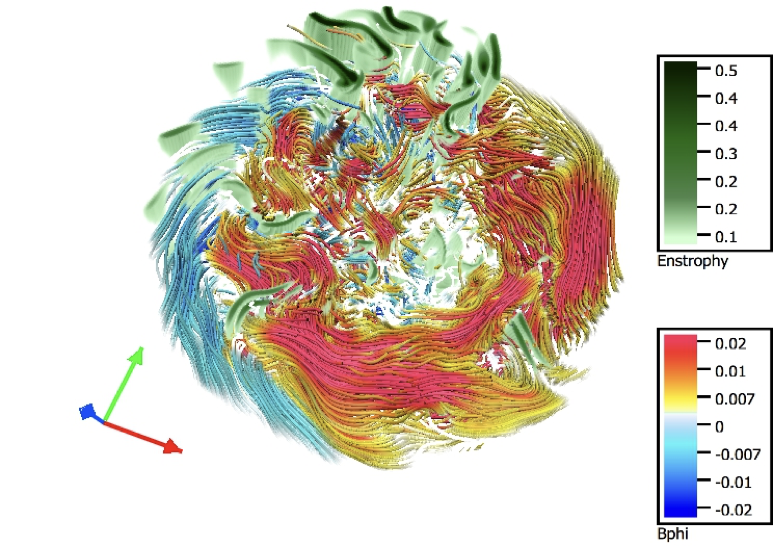
\includegraphics[width=0.21\textwidth]{./figs/mdwarf.png}
	\vspace{-16pt}
	\end{center}
    \caption{A volume rendering of a global dynamo simulation in Dedalus.
	Enstrophy, or the magnitude of vorticity, is shown in green.
	Red and blue lines denote the magnitude and direction of azimuthal magnetic field.
	\label{fig:mdwarf} }
\end{wrapfigure}
During my time at Stanford, I will extend my accelerated evolution method \citep{anders&all2018} to the evolution of thermodynamic and angular momentum profiles in global simulations.
Dedalus is capable of accurately simulating global domains which include the origin at $r = 0$ \citep{lecoanet&all2019}; a visualization of basic outputs from these simulations is shown in Fig.~\ref{fig:mdwarf}.
The large-scale structures seen in Fig.~\ref{fig:mdwarf} arise quickly, but the equilibration and saturation of these structures and other simulation measurements often takes KH timescales which cannot be feasibly simulated in turbulent regimes.
I will design a generalized public module which can accelerate mean profiles and flows in global simulations.
This module will read in statistical measures from unequilibrated convective simulations and output the properly equilibrated mean state.
Researchers simulating convection with Dedalus or other codes will be able to use this module to rapidly equilibrate simulations with state-of-the-art turbulent dynamics.
This tool will benefit numericists across diverse research fields, such as those who study general circulation models (GCMs) in the atmospheres of the Earth and exoplanets or modelers of dynamo processes in planetary cores and stellar atmospheres.
Once completed, I will use this tool in my own research to accelerate the evolution of highly turbulent, solar-like simulations to understand the nature of global flows and dynamos in an equilibrated simulation.
I look forward to collaborating on this project with experts in global convective simulations like Princeton's Prof.~Adam Burrows as well as GFDL's many GCM experts.


\vspace{-10pt}
\section*{How Stanford enables these accomplishments}
\vspace{-8pt}
Stanford University and the Stanford Science Fellowship would give me the freedom to study these ambitious problems in astrophysical fluid dynamics.
The projects proposed here seek to understand stellar convection from small to global scales and build naturally upon my PhD research.
These projects help solve exciting problems in stellar structure with applications in numerous astrophysical subdisciplines.

Stanford is the perfect location for carrying out this work due to the opportunities available for interdisciplinary collaboration between astrophysicists, geophysical fluid dynamicists, and applied mathematicians.
The most natural collaborator on this work proposed here is Prof.~Tom Abel of Stanford's physics department and the SLAC National Accelerator Laboratory; his expertise in astrophysical fluid dynamics and scientific visualization, as well as his broad interest on astrophysical topics would make him an excellent mentor as I tackle these problems and grow as a researcher.
From Prof.~Abel's group, I would collaborate with the numerous experts in Stanford's Physics department, such as Prof.~Petrosian, who has recently studied the hydrodynamics of solar flares, Prof.~Wagoner, who has studied waves in astrophysical accretion disks.
I would also aim to collaborate on experts on atmospheric and oceanic processes in Stanford's School of Earth, Energy \& Environmental Sciences department, such as Profs.~Sheshadri and Thomas, as many fundamental fluid dynamical processes in stars play roles in the Earth's atmospheres and oceans.
Furthermore, experts in Stanford's Mathematics departments with experience in fluid flows (e.g., Profs.~Ryzhik and Tokieda), numerical methods (e..g, Prof.~Kazeev) will be expert collaborators while I ensure that my numerical methodologies and theories are sound.
Stanford's Center for Turbulence Research, which houses many experts on turbulent fluid dynamics such as Prof.~Javier Jim\'{e}nez, will create numerous opportunities for cross-disciplinary collaboration as I carry out my research plan.
I look forward to the opportunity to create cross-disciplinary collaborations and carry on Stanford's excellent research tradition while making lasting contributions which help solve the Convective Conundrum and other fascinating problems. 

\bibliographystyle{yahapj}
\bibliography{biblio}
\end{document}
